\documentclass[../MathsNotesBase.tex]{subfiles}

\date{\vspace{-6ex}}

\begin{document}
	
	\pagebreak
	\searchableSection{Affine Spaces and Transformations}{linear algebra}{
		\bigskip\bigskip
		\subsubsection{Affine Spaces}
		\boxeddefinition{An \textbf{affine space} is a generalization of a Euclidean space in which there is no particular point designated as the origin. As a result vectors can be viewed as displacements rather than points.\\\\
			Let $V$ be a vector space and $P$ be a set of points. Then we can form an affine space over $V$ and $P$ by defining the vectors in $V$ as displacements connecting members of $P$ such that, for ${ Q_1,Q_2 \in P,\, \v \in V }$,
			\[ Q_1 + \v = Q_2 \iff Q_2 - Q_1 = \v \iff Q_1 - Q_2 = -\v. \]
		}
		\boxeddefinition{A \textbf{frame} of an affine space is an extension of a basis of its underlying vector space to include a point designated as an origin. If ${ \v_1,\dots,\v_n }$ is a basis of a vector space $V$ and $Q$ is a point in the set of points $P$, then ${ F = (\v_1,\dots,\v_n, Q) }$ is a frame of the affine space over $V$ and $P$.}
		\boxeddefinition{The \textbf{dimension} of an affine space is the dimension of the underlying vector space.}
		
		\bigskip
		\labeledProposition{Any linear combination of points in an affine space where the coefficients sum to 0 results in a vector.}{sum_affine_points_with_coeffs_sum_to_zero_are_vectors}
		\begin{proof}
			Let $S$ be a sum of $n$ points ${ Q_i \in P }$ in an affine space associated with a vector space $V$ such that,
			\[ S = \sum_{i=0}^n \alpha_i Q_i  \eqand \sum_{i=0}^n \alpha_i = 0. \]
			Then, if we take the partial sum of the first two points,
			\[ S_2 = \alpha_1 Q_1 + \alpha_2 Q_2 = \alpha_1(Q_1 - Q_2) + (\alpha_1 + \alpha_2)Q_2 \]
			and then the next partial sum of the first three points,
			\begin{align*}
				S_3 &= \alpha_1(Q_1 - Q_2) + (\alpha_1 + \alpha_2)Q_2 + \alpha_3 Q_3 \\
				&= \alpha_1(Q_1 - Q_2) +  (\alpha_1 + \alpha_2)(Q_2 - Q_3) +  (\alpha_1 + \alpha_2 + \alpha_3) Q_3
			\end{align*}
			we can see that, by induction, the $n$th sum is,
			\begin{align*}
				S &= \alpha_1(Q_1 - Q_2) \\
				&\hspace{20pt} + (\alpha_1 + \alpha_2)(Q_2 - Q_3)\\
				&\hspace{20pt} + (\alpha_1 + \alpha_2 + \alpha_3)(Q_3 - Q_4)\\
				&\hspace{24pt} \vdots\\
				&\hspace{20pt} + (\alpha_1 + \cdots + \alpha_{n-1})(Q_{n-1} - Q_n)\\
				&\hspace{20pt} + (\alpha_1 + \cdots + \alpha_n)Q_n.
			\end{align*}
			But we have ${ \alpha_1 + \cdots + \alpha_n = 0 }$ so the final term is 0. As a result $S$ is a summation of terms of the form,
			\[ (\alpha_1 + \cdots + \alpha_{i-1})(Q_{i-1} - Q_i) \]
			where ${ Q_{i-1} - Q_i }$ is a vector. Therefore $S$ is a linear combination of vectors in $V$ and is therefore also a vector in $V$.
		\end{proof}
		\begin{corollary}
			\label{coro:sum_affine_points_with_coeffs_sum_to_one_are_vectors}
			Any linear combination of points in an affine space where the coefficients sum to 1 results in a point.
		\end{corollary}
		\begin{proof}
			In the preceding proof if we had, instead, ${ \alpha_1 + \cdots + \alpha_n = 1 }$ then the final term would equal $Q_n$ and the resulting summation would be a vector plus the point $Q_n$. Therefore the sum is a point.
		\end{proof}
		
		\pagebreak
		\subsubsection{Intuition of Affine Spaces}
		\begin{wrapfigure}{l}{0.5\textwidth}
			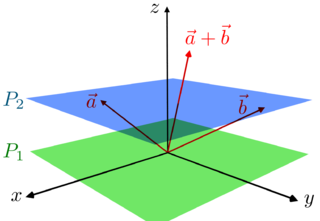
\includegraphics[width=0.9\linewidth]{\resourceDir/img/320px-Affine_space_R3.png} 
			\label{fig:affine_space_schematic}
		\end{wrapfigure}
		A translated linear subspace of a vector space like $P_2$ above that no longer passes through the origin is referred to as an \textbf{affine subspace}. It is not a vector space as ${ \0 \notin P_2 }$ and ${ \V{a},\V{b} \in P_2 }$ but ${ \V{a} + \V{b} \notin P_2 }$. 
		However, if we instead consider displacements between points --- e.g. ${ \V{b} - \V{a} }$ --- then we see the relationship between affine spaces and vector spaces: ${ \V{b} - \V{a} \in P_1 }$. The displacements between points in $P_2$ form a linear subspace. So we can define an affine space $A$ based on the set of points in $P_2$ and the vectors in $P_1$.
		
		
		\bigskip
		\subsubsection{Affine Combinations}
		\boxeddefinition{An \textbf{affine combination} of vectors is a combination such that the coefficients sum to 1.}
		\note{The definition of an affine combination differs from that of a convex combination in that the coefficients of a convex combination are additionally required to be non-negative.}
		
		\bigskip
		In an affine space there is no particular point designated as the origin but we can describe vector displacements between points as an ordered pair of points, for example, ${ (p,a) = \V{pa} }$. Affine combinations of displacements agree on the resulting point with linear combinations in the corresponding Euclidean space.\\
		For example, imagine a point $p$ in an affine space is at coordinates ${ (-1,4) }$ in the corresponding Euclidean space and similarly points $a$ and $b$ are at ${ (3,4) }$ and ${ (6,1) }$ respectively. Then, if we take an affine combination of the displacements to $a$ and $b$ the resulting point is independent of the chosen origin point.
		%	\begin{wrapfigure}{l}{0.5\textwidth}
		%		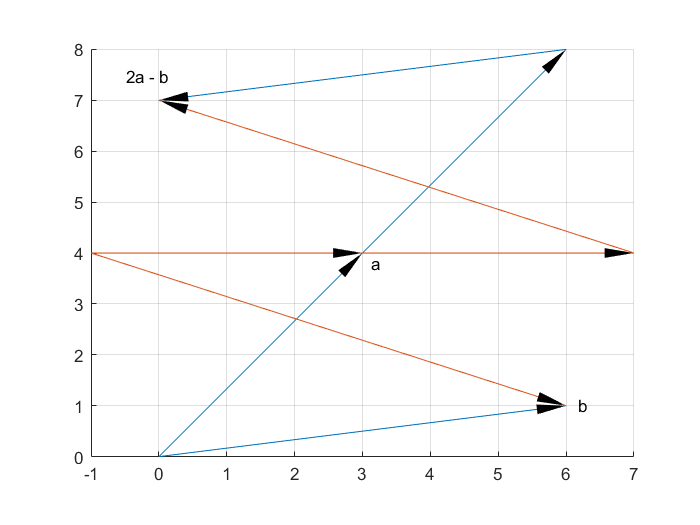
\includegraphics[width=\linewidth]{\resourceDir/img/affine_combinations_example.png} 
		%		\label{fig:affine_combinations_example}
		%	\end{wrapfigure}
		%	
		
		\begin{figure}[h!]
			\centering
			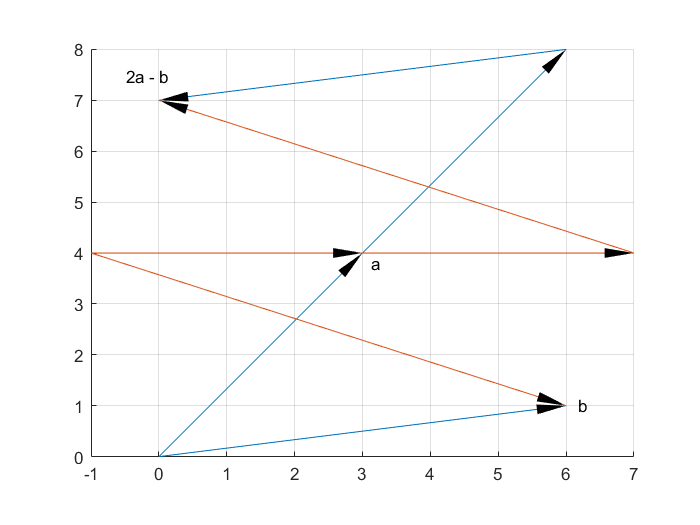
\includegraphics[width=300px]{\resourceDir/img/affine_combinations_example.png}
			\caption{\small The diagram shows the affine combination ${ 2\V{a} - \V{b} = 2\V{pa} - \V{pb} }$ where $\V{a}$ denotes the usual position vector in the Euclidean space.}
			\label{fig:affine_combinations_example}
		\end{figure}
		
		
		
		\bigskip\bigskip\bigskip
		\subsubsection{Affine Transformations}
		\boxeddefinition{Let ${ T: A_1 \longmapsto A_2 }$ be a mapping between the affine spaces $A_1$ and $A_2$. Then $T$ is an \textbf{affine transformation} if:
			\begin{itemize}
				\item{$T$ maps vectors to vectors and points to points.}
				\item{$T$ is a linear transformation over the vectors in the underlying vector space.}
				\item{${ T(Q + \v) = T(Q) + T(\v) }$.}
			\end{itemize}
		}
		
		\medskip
		\note{In an affine space a \textbf{translation} can be regarded as a change of frame in which we \textbf{change the origin point} while the vector basis may remain unchanged.}
		
		\medskip
		\labeledProposition{Affine transformations preserve parallelism.}{affine_transformations_preserve_parallelism}
		\begin{proof}
			Let $A$ be an affine space defined over a set of points $P$ and a vector space $V$ and let ${ Q_1,Q_2 \in P }$ and ${ \v \in V }$. Then, for ${ s,t \in \F{} }$,
			\[ l_1 = Q_1 + t\v \eqand l_2 = Q_2 + s\v \]
			are parallel lines in $A$. Let $T$ be an arbitrary affine transformation over $A$. Then,
			\[ l_1' = T(l_1) = T(Q_1) + tT(\v) \eqand l_2' = T(l_2) = T(Q_2) + sT(\v) \]
			are also parallel.
		\end{proof}
		
		\medskip
		\labeledProposition{An affine transformation that preserves the dot product is left multiplication by an orthogonal matrix.}{dot-product-preserving-affine-trans-is-left-mult-by-ortho-matrix}
		\begin{proof}
			Firstly, note that if a transformation $m$ preserves the dot product and also fixes the standard basis vectors $\e{i}$ then,
			\[ m(\e{i}) = \e{i} \eqand x_i = \x \dotprod \e{i} = m(\x) \dotprod m(\e{i}) = m(\x) \dotprod \e{i} = m(\x)_i. \]
			Therefore, such a transformation $m$ is the identity transformation.\\
			Now, assume a transformation $m'$ preserves the dot product (but does not necessarily fix the standard basis vectors) in $\R{n}$ and let 
			\[ B' = \{ m'(\e{1}),\dots,m'(\e{n}) \} \]
			be the transformed standard basis vectors. Then, if $[B']$ is the matrix whose columns are the elements of $B'$ then, because $m'$ preserves the dot product, $[B']$ is an orthogonal matrix as, by \autoref{prop:orthogonal-matrices-are-subgroup}, is $\inv{[B']}$. So, composing this with $m'$,
			\[ m'' = \inv{[B']}m' \]
			is a transformation that both preserves the dot product and fixes the standard basis vectors. Therefore we have,
			\[ m'' = I_n = \inv{[B']}m' \iff [B'] = m' \]
			so that $m'$ is left multiplication by $[B']$, an orthogonal matrix.
		\end{proof}
		
		\bigskip\bigskip
		\subsubsubsection{Properties of affine transformations}
		We can characterize affine transformations according to their form and behaviour in the Euclidean spaces $\R{2}$ and $\R{3}$. Specifically, whether the transformation:
		\begin{enumerate}
			\item{Fixes the origin: ${ T(\0) = \0 }$}
			\item{Preserves the dot product: ${ T(\v)\dotprod T(\w) = \v\dotprod\w }$, matrix is orthogonal}
			\item{Preserves distances: ${ \norm{T(\v) - T(\w)} = \norm{\v - \w} }$}
			\item{Preserves angles: matrix is scalar multiple of orthogonal matrix}		
			\item{Preserves orientation: transformation does not include a reflection, determinant of matrix is positive}
			\item{Preserves parallelism: transformation exhibits affine property (linearity under affine combinations)}
		\end{enumerate}
		
		As we can see here, the property of preserving parallelism depends only on the affine property so clearly, all affine transformations exhibit this behaviour. As a consequence of preserving parallelism, affine transformations preserve the dimension of affine subspaces (points, lines, planes, etc.). They do not preserve distances between points however, but they do preserve ratios of distances between points lying on a straight line.\\
		
		\bigskip
		\subsubsubsection{Classes of affine transformations}
		The most common subclassifications of affine transformations are:
		\begin{itemize}
			\item{Linear: preserves the origin.}
			\item{Conformal: preserves angles.}
			\item{Isometry (also known as a congruent transformation): preserves distances in metric spaces and so also implicity, angles. In a Euclidean space these transformations are known as a Euclidean isometries or rigid transformations.}
			\item{Rigid Motion: Euclidean isometry / rigid transformation that also preserves orientation.}
		\end{itemize}
		
		\bigskip
		\subsubsection{Isometries}
		\bigskip
		A Euclidean isometry or rigid motion, for example, carries a triangle to a congruent triangle. So, it preserves distances and angles but not necessarily orientation (a reflection flips the orientation).\\
		The composition of two rigid motions is a rigid motion and the inverse of a rigid motion is also a rigid motion. Therefore, the rigid motions of $\R{n}$ form a group under composition of operations. This group is called the \textit{group of motions} and denoted $M_n$.
		
		\bigskip
		\labeledProposition{A rigid motion that fixes the origin preserves the dot product.}{non-translational-isometries-preserve-dot-product}
		\begin{proof}
			Let $m$ be a rigid motion that fixes the origin. Then $m$ is an isometry and so preserves distances and also $m$ maps the origin to the origin. So we have,
			\[ \norm{m(\v) - m(\w)} = \norm{\v - \w} \eqand m(\0) = \0. \]
			We can rewrite the isometry property as,
			\begin{align*}
				&& \sqrt{(m(\v) - m(\w))\dotprod(m(\v) - m(\w))} &= \sqrt{(\v - \w)\dotprod(\v - \w)}\\
				&\iff & (m(\v) - m(\w))\dotprod(m(\v) - m(\w)) &= (\v - \w)\dotprod(\v - \w). &\sidecomment{}
			\end{align*}
			Now, if we take the case where ${ \w = \0 = m(\w) }$,
			\begin{align*}
				&& (m(\v) - \0)\dotprod(m(\v) - \0) &= (\v - \0)\dotprod(\v - \0) \\
				&\iff & m(\v) \dotprod m(\v) &= \v \dotprod \v. &\sidecomment{}
			\end{align*}
			and we can deduce that ${ m(\x) \dotprod m(\x) = \x \dotprod \x }$ for any vector $\x$. Using this along with the properties of the dot product we obtain,
			\begin{align*}
				&& (m(\v) - m(\w))\dotprod(m(\v) - m(\w)) &= (\v - \w)\dotprod(\v - \w) \\
				&\iff & m(\v)\dotprod m(\v) + m(\w)\dotprod m(\w) - 2m(\v)\dotprod m(\w) &= \v\dotprod\v + \w\dotprod\w - 2\v\dotprod\w &\sidecomment{} \\
				&\iff & -2m(\v)\dotprod m(\w) &= -2\v\dotprod\w &\sidecomment{} \\
				&\iff & m(\v)\dotprod m(\w) &= \v\dotprod\w. &\sidecomment{}
			\end{align*}
			
			Therefore, $m$ preserves the dot product and, by \autoref{prop:dot-product-preserving-affine-trans-is-left-mult-by-ortho-matrix}, is left multiplication by an orthogonal matrix.
		\end{proof}
		\begin{corollary}
			\label{coro:isometry-fixes-origin-left-mult-by-orthogonal-matrix}
			A rigid motion that fixes the origin is left multiplication by an orthogonal matrix and, therefore, also a linear operator.
		\end{corollary}
		
		\medskip
		\labeledProposition{Left multiplication by any orthogonal matrix is a Euclidean isometry (a rigid motion) that fixes the origin.}{left-mult-by-ortho-matrix-is-rigid-motion}
		\begin{proof}
			By, \autoref{prop:left_mult_by_ortho_matrix_preserves_dot_product}, left multiplication by an orthogonal matrix preserves the dot product. So, if $m$ is an affine transformation such that ${ m(\x) = A\x  }$ where $A$ is an orthogonal matrix then,
			\begin{align*}
				&& \norm{m(\v - \w)}^2 = m(\v - \w)\dotprod m(\v - \w) &= (\v - \w)\dotprod (\v - \w) = \norm{\v - \w}^2 \\
				&\iff & \norm{m(\v - \w)} &= \norm{\v - \w} &\sidecomment{} \\
			\end{align*}
			But also, left multiplication by a matrix is a linear operator so ${ m(\v - \w) = m(\v) - m(\w) }$ meaning that,
			\[ \norm{m(\v - \w)} = \norm{m(\v) - m(\w)} = \norm{\v - \w} \]
			which is the isometry property for $m$.
		\end{proof}
		
		
		\bigskip\bigskip
		\subsubsubsection{Linear}
		Isometries that fix the origin are linear operators and rigid motions in Euclidean space.\\
		
		
		\bigskip
		\subsubsubsection{Translation}
		If $T$ is a translation then, in general, ${ T(\0) \neq \0 }$ so translations do not fix the origin and, as a result, are \textbf{not} linear transformations. However, translations preserve distances and angles (and orientation because there is no reflection) so they are rigid motions. For example:
		\begin{exe}
			\ex{Let ${ \v = (v_1,\dots,v_n) }$ be any fixed vector in $\R{n}$. Then translation by $\v$ is the map,
				\[ t_v(\x) = \x + \v = \begin{bmatrix}x_1 + v_1\\\vdots\\x_n + v_n\end{bmatrix} \]
				which can be seen to be isometric (a rigid transformation) by,
				\begin{align*}
					&& t_v(\x) - t_v(\V{y}) = (\x + \v) - (\V{y} +\v) &= \x - \V{y} \\
					&\implies & \norm{t_v(\x) - t_v(\V{y})} &= \norm{\x - \V{y}}. &\sidecomment{}
				\end{align*}
			}
		\end{exe}
		
		\medskip
		\labeledProposition{Every rigid motion $m$ is the composition of an orthogonal linear operator and a translation. In other words, for some orthogonal matrix $A$ and fixed vector $\v$, it takes the form,
			\[ m(\x) = A\x + \v. \]
		}{every_rigid_motion_is_linear_op_plus_translation}
		\begin{proof}
			Let ${ \v = m(\0) }$ and ${ t_v(\x) = \x + \v }$ with inverse ${ t_{-v}(\x) = \x - \v }$. Then composing this with $m$, the resulting transformation,
			\[ (t_{-v} \circ m)(\x) = m(\x) - \v \]
			continues to be isometric --- because it is the composition of isometric transformations --- and it fixes the origin because ${ (t_{-v} \circ m)(\0) = m(\0) - \v = m(\0) - m(\0) = \0 }$. It is therefore, by \autoref{coro:isometry-fixes-origin-left-mult-by-orthogonal-matrix}, left multiplication by an orthogonal matrix. So we can represent it as,
			\[ (t_{-v} \circ m)(\x) = t_{-v}(m(\x)) = A\x. \]
			Since ${ t_{-v} = \inv{t_v} }$ we can apply $t_{v}$ to both sides of the equation,
			\[ m(\x) = t_{v}(A\x) = A\x + \v. \]
			The obtained representation is uniquely determined by $m$ as ${ \v = m(\0) }$ is clearly unique and then the translation $t_{-v}$ is uniquely determined by $\v$ and then ${ A = (t_{-v} \circ m) }$ is unique for a given $\v$ and $m$.
		\end{proof}
		
		\medskip\note{For a rigid motion ${ m(\x) = A\x + \v }$, $m$ is orientation-preserving if the matrix $A$ is orientation-preserving and orientation-reversing if $A$ is orientation-reversing.}
		
		\bigskip
		\subsubsubsection{Rotation}
		Rotations preserve distances, angles and orientation and so are rigid motions. Rotations also fix a vector which is known as the axis of rotation. If the axis of rotation contains the origin then they fix the origin and so are linear operators.
		
		\medskip
		\labeledTheorem{The rotations of $\R{2}$ and $\R{3}$ about the origin are the linear operators whose matrices with respect to the standard basis are orthogonal and have determinant 1.}{rotations-of-r2-r3-about-origin-are-ortho-mat-det-1}
		\begin{proof}
			A rotation about the origin $m$ involves rotating the standard basis vectors through an angle $\theta$. It is in the definition of this rotation that the image of the standard basis vectors continue to subtend the same angle, ${ \pi/2 }$. Therefore, the rotation must preserve angles. It is also part of the definition that the image under rotation is not scaled so the rotation must preserve distances and must be a congruent transformation. Since the axis of rotation passes through the origin the origin is unchanged by this rotation and so these rotations are rigid motions that fix the origin and have the form,
			\[ m(\x) = A\x \]
			where $A$ is an orthogonal matrix. Additionally, rotations do not change the orientation of an shape and so their matrices have determinant 1.
		\end{proof}
		
		\medskip
		\note{The rotation matrices --- orthogonal matrices with determinant 1 --- form a subgroup of the group $O_n$ of orthogonal matrices called the \textbf{special orthogonal group} and denoted $SO_n$.}
		
		\labeledProposition{Every member of the special orthogonal group ${ A \in SO_2 }$ is the matrix of a rotation.}{all-members-SO2-are-rotations}
		\begin{proof}
			Let ${ A \in SO_2 }$. Then $A$ is a ${ 2 \times 2 }$ orthogonal matrix with determinant 1. Let $\v_1$ be the first column of $A$ which, since $A$ is orthogonal, is a unit vector. Now assume that $R$ is the matrix of a rotation whose first column is $\v_1$ --- which is possible because $\v_1$ is a unit vector so $R$ can be orthogonal. Then the matrix
			\[ B = \inv{R}A \]
			fixes $\e{1}$ and also, as the composition of two orthogonal vectors, is orthogonal. Therefore the second column of $B$ is a unit vector orthogonal to $\e{1}$ which could be $\e{2}$ or $-\e{2}$. 
			
			However, $R$ is an orthogonal matrix with determinant 1 and so is a member of $SO_2$ which means that ${ \inv{R}A = B }$ is also in $SO_2$. 
			
			This, in turn, means that $B$ has determinant 1 which implies that the second column of $B$ is not $-\e{2}$ and is, therefore, $\e{2}$. So, we have obtained the result that ${ B = I = \inv{R}A }$ which implies that ${ R = A }$.
		\end{proof}
		
		\bigskip
		\subsubsubsection{Rotating $\bm{\R{2}}$ about the origin}
		Rotating the 2-d plane about the origin means that the axis of rotation is just the origin (so the fixed vector is $\0$).
		
		For example:
		\begin{exe}
			\ex{A rotation $\rho_{\theta}$ of the plane through an angle $\theta$ is a linear operator on $\R{2}$ whose matrix with respect to the standard basis is
				\[ R = 	\begin{bmatrix}
					\cos\theta & -\sin\theta\\
					\sin\theta & \cos\theta
				\end{bmatrix}.
				\]
				We can see that this is a rotation if we take ${ \x = (x_1,x_2)^T \in \R{2} }$ and write it in polar coordinates,
				\[ \x = (r,\alpha). \]
				So, relating the polar and rectangular coordinates,
				\[ \x = (r\cos\alpha, r\sin\alpha)^T. \]
				When we left-multiply by $R$,
				\begin{align*}
					R\x &= \begin{bmatrix}
						\cos\theta & -\sin\theta\\
						\sin\theta & \cos\theta
					\end{bmatrix}
					\begin{bmatrix}
						r\cos\alpha\\
						r\sin\alpha
					\end{bmatrix} \\
					&= \begin{bmatrix}
						r\cos\alpha\cos\theta - r\sin\alpha\sin\theta\\
						r\cos\alpha\sin\theta + r\sin\alpha\cos\theta
					\end{bmatrix} \\
					&= 	\begin{bmatrix}
						r\cos{(\alpha + \theta)}\\
						r\sin{(\alpha + \theta)}
					\end{bmatrix}.
				\end{align*}
				Note that $R$ is orthogonal because
				\[  \begin{bmatrix}
					\cos\theta\\
					\sin\theta
				\end{bmatrix} \dotprod 
				\begin{bmatrix}
					-\sin\theta\\
					\cos\theta
				\end{bmatrix} = -\cos\theta\sin\theta + \sin\theta\cos\theta = 0 \]
				and ${ det\,R = 1 }$,
				\[ 
				\begin{vmatrix}
					\cos\theta & -\sin\theta\\
					\sin\theta & \cos\theta
				\end{vmatrix} = \cos^2\theta + \sin^2\theta = 1.
				\]
			}
		\end{exe}
		
		\bigskip
		\subsubsubsection{Rotating $\bm{\R{3}}$ about the origin}	 
		\boxeddefinition{Define $\rho$ as a rotation in $\R{3}$ around the origin if:
			\begin{enumerate}[label=(\roman*)]
				\item{$\rho$ is a rigid motion (orientation-preserving Euclidean isometry) that fixes the origin;}
				\item{$\rho$ also fixes a nonzero vector $\v$;}
				\item{$\rho$ operates as a rotation on the plane $P$ orthogonal to $\v$.}
		\end{enumerate}}
		\note{Note that this definition could be described as selecting a 2-dimensional subspace of $\R{3}$ and performing a 2-dimensional rotation on it as if it were $\R{2}$.}
		Condition (i) implies, by \autoref{coro:isometry-fixes-origin-left-mult-by-orthogonal-matrix}, that $\rho$ is left multiplication by an orthogonal matrix. Condition (ii) states that $\rho$ has an eigenvector $\v$ with eigenvalue 1. Then, because $\rho$ preserves angles, the plane $P$ referenced in condition (iii) that is orthogonal to the eigenvector $\v$, must map to a plane that is orthogonal to the map of $\v$ in the image of $\rho$. But $\v$ is fixed by $\rho$ and is unchanged in the image. Also $\v$ uniquely identifies a plane orthogonal to it. Therefore the plane $P$ is unchanged in the image also. In other words, $P$ is an invariant subspace. So, condition (iii) says that the restriction of $\rho$ to this invariant subspace is a rotation.
		
		\bigskip
		For example:
		\begin{exe}
			\ex{A rotation of $\R{3}$ about the origin can be described by a pair $(\v, \theta)$ consisting of a unit
				vector $\v$, a vector of length 1, which lies in the axis of rotation, and a nonzero angle
				$\theta$, the angle of rotation. The two pairs $(\v, \theta)$ and $(-\v, -\theta)$ represent the same rotation.
				We also consider the identity map to be a rotation, though its axis is indeterminate.\\
				The matrix representing a rotation through the angle $\theta$ about the vector $\e{1}$ is obtained easily from the $2 \times 2$ rotation matrix. It is
				\[ A = \begin{bmatrix}
					1 & 0 & 0\\
					0 & \cos\theta & -\sin\theta\\
					0 & \sin\theta & \cos\theta
				\end{bmatrix}.
				\]
				Multiplication by $A$ fixes the first coordinate $x_1$ of a vector and operates by rotation on $(x_2, x_3)^T$. All rotations of $\R{3}$ are linear operators, but their matrices can be fairly complicated.
			}
		\end{exe}
		
		\bigskip
		\labeledProposition{Every element of $SO_3$ has eigenvalue 1.}{elements-of-SO3-have-eigenvalue-1}
		\begin{proof}
			Let ${ A \in SO_3 }$. Then $A$ is an orthogonal ${ 3 \times 3 }$ matrix with determinant equal to 1. Reasoning from orthogonality of $A$ we have,
			\begin{align*}
				&& A^TA &= I \\
				&\iff & A^TA - A^T &= I - A^T &\sidecomment{} \\
				&\iff & A^T(A - I) &= I - A^T &\sidecomment{} \\
				&\iff & A^T(A - I) &= (I - A)^T. &\sidecomment{by \autoref{prop:matrix-transpose-distributes-over-addition}}
			\end{align*}
			If we take the determinants of both sides of this equation we obtain,
			\begin{align*}
				&& det(A^T)\cdot det(A - I) &= det((I-A)^T) &\sidecomment{by \autoref{prop:determinant_of_matrix_product}} \\
				&\iff & det(A)\cdot det(A - I) &= det(I - A) &\sidecomment{by \autoref{prop:determinant_of_matrix_equal_to_its_transpose}} \\
				&\iff & det(A - I) &= det(I - A). &\sidecomment{${ det(A) = 1 }$}
			\end{align*}
			But the dimension of $A$ being 3 implies that
			\[ det(-A) = (-1)^3 det(A) = -det(A) \]
			so that,
			\[ det(A - I) = det(I - A) \iff det(A - I) = 0. \]
			Therefore $A$ has the eigenvalue 1.
		\end{proof}
		
		\bigskip
		\labeledProposition{The elements of $SO_3$ are precisely the rotations about the origin of $\R{3}$.}{elements-of-SO3-are-the-rotations-around-origin-in-R3}
		\begin{proof}
			Let ${ \rho: \R{3} \longmapsto \R{3} }$ be defined as ${ \rho(\x) = A\x }$ where ${ A \in SO_3 }$. Then,
			\begin{itemize}
				\item{by \autoref{prop:left-mult-by-ortho-matrix-is-rigid-motion} and orthogonality of ${ A \in SO_3 }$, left multiplication by $A$ is a rigid motion that fixes the origin. So $\rho$ is isometric and fixes the origin;}
				\item{\autoref{prop:elements-of-SO3-have-eigenvalue-1} shows that every ${ A \in SO_3 }$ has eigenvalue 1 which implies that $\rho$ fixes a nonzero vector;}
				\item{if we let $\v$ be the nonzero vector fixed by $\rho$ (i.e. its eigenvector with eigenvalue 1), then we can normalize it to find the unit vector parallel to $\v$, say $\u_1$. Next we can find two unit vectors orthogonal to $\u_1$ --- say $\u_2$ and $\u_3$ --- and these must be a basis for the plane orthogonal to $\v$. Furthermore, if we select $\u_2$ and $\u_3$ to be orthogonal to each other than ${ B = \{\u_1,\u_2,\u_3\} }$ is an orthonormal basis of $\R{3}$.\\
					Now if we define ${ P = \inv{[B]} }$ then,
					\[ A' = \inv{P}AP \]
					is similar to the matrix $A$ and so has the same determinant, 1. Furthermore, because $B$ is an orthonormal basis, the matrices ${ [B],\, \inv{[B]} = P }$ are orthogonal. Since both $P$ and $A$ are orthogonal, ${ \inv{P}AP = A' }$ is orthogonal also. Since $A'$ is orthogonal and has determinant equal to 1, it is a member of $SO_3$.\\
					If we examine the structure of $A'$, we see that the first column of $A'$ is $\v_1$ --- the unit vector in the direction of $\v$. Since $\v$ is an eigenvector of $\rho$ with eigenvalue 1, the first column of $A'$ is $\e{1}$ and since $A'$ is orthogonal, the other columns are orthogonal to the first. So the block structure of $A'$ looks like,
					\[ A' = \begin{bmatrix}
						1 & 0 \\
						0 & R
					\end{bmatrix} 
					\]
					where $R$ is a ${ 2 \times 2 }$ matrix.\\
					We know that the determinant of $A'$ is 1 and this implies that the determinant of $R$ is also 1. Furthermore, $R$ must also be orthogonal and so ${ R \in SO_2 }$. So, by \autoref{prop:all-members-SO2-are-rotations}, $R$ is a rotation. Therefore $R$ represents a rotation of the plane orthogonal to $\v$ and this implies that $\rho$ rotates the plane orthogonal to $\v$ as required.
				}
			\end{itemize}
		\end{proof}
		
		\bigskip
		\subsubsubsection{Uniform Scaling}
		Uniform scaling is a scalar multiple of an orthogonal matrix and is therefore a linear operator which means that it fixes the origin. It also preserves angles but not distances between points.
		
		
		\bigskip\bigskip
		\subsubsection{Conformal Transformations}
		\bigskip
		\subsubsubsection{Non-uniform Scaling}
		Non-uniform scaling, however, its matrix is not a scalar multiple of an orthogonal matrix and, as such, it does not preserve angles. An important example is:
		\begin{exe}
			\ex{\textbf{Mercator projection}:\\\\
				This is a map projection that was designed so that rhumb lines (lines of constant bearing over the surface of the earth) are straight lines on the map. To achieve this the projection ensures that a square on the surface of the earth presents as a square on the map.\\
				Then, modelling the earth as a sphere of radius $R$, if lines of latitude are horizontal grid lines across the map, then each actual line of latitude with circumference ${ 2\pi R \cos\phi }$ where $\phi$ is the angle of latitude will present on the map as the same length as the equator, which in reality is ${ 2\pi R }$. So they appear to be a line of length ${ \cos\phi }$ times longer than they actually are, i.e. they are stretched by ${ \sec{\phi} }$.\\
				So, the map projection will stretch the width of a square on the surface of the earth by ${ \sec{\phi} }$ and to maintain it as a square, it is necessary to stretch the height of the square by the same amount, ${ \sec{\phi} }$. The actual square on the surface of the earth has height (approximately for a small square) ${ R\Delta\phi }$ so, on the map we need a height ${ \Delta y \propto \Delta\phi\sec\phi }$. Therefore, we have,
				\[ \frac{dy}{d\phi} = \sec\phi \implies y = \ln{(\tan\phi + \sec\phi)} + c \]
				where $c$ is a constant that we can set to 0. 
				See \url{https://www.math.ubc.ca/~israel/m103/mercator/mercator.html} for a description of this derivation. For more information on conformal map projections generally see: \href{https://arxiv.org/pdf/1412.7690.pdf}{Map Projection, York University, Toronto} and \href{http://diposit.ub.edu/dspace/bitstream/2445/121898/2/memoria.pdf}{Conformal Cartographic
					Representations - University of Barcelona}.
			}
		\end{exe}
		
		\subsubsubsection{Reflection}
		Reflection usually refers to a Euclidean Isometry (rigid transformation over a Euclidean space) that fixes a hyperplane (so a line in $\R{2}$ and a plane in $\R{3}$) but does not preserve orientation so is not a rigid motion. However, it may also refer to a transformation that fixes an affine space of lower dimension than a hyperplane --- for example, reflection in a point --- in which case it does preserve orientation and is, therefore, a rigid motion (in fact, reflection in the origin in $\R{2}$ is equal to rotation by $\pi$). Reflection may fix the origin or may not, depending on whether or not the origin is contained in the affine space fixed by the reflection.
		
		\bigskip
		\subsubsection{Non-Rigid non-Conformal Transformations}
		\bigskip
		\subsubsubsection{Shear}
		Shear neither preserves distances nor angles. It does preserve parallelism though (as do all affine transformations) and it also fixes the origin, so it is a linear operator.
		
		\bigskip\bigskip
		\note{For more in-depth treatment of affine spaces and transformations see:
			\begin{itemize}
				\item{First two lectures of \href{https://web.ma.utexas.edu/users/dafr/M375T/}{University of Texas - Multivariable Analysis}.}
				\item{\url{https://www.maa.org/sites/default/files/pdf/pubs/books/meg/meg_ch12.pdf}}
			\end{itemize}
		}
	
	}

\end{document}